\chapter{Testing Strategy and Results}
\section{Strategy for Gathering of Results}
The experiments were conducted through the simulation of a group of nodes on a single computer. The accuracy of each node was evaluated on an unseen test set and subsequently recorded in a file after each training step. All nodes shared the same test set. Below are the specific details of the running of each experiment:
\begin{description}
	\item [Chosen Metric: Accuracy:] The metric chosen for the following experiments was accuracy, due to its comprehensible nature. Despite the fact that an unbalanced dataset presents one of the significant drawbacks of using accuracy, this concern is irrelevant in the case of MNIST-F since it is a balanced dataset, meaning it has the same number of samples in each class. The accuracy of each node is computed after each training step using the test subset of MNIST-F, and none of the nodes are ever provided access to the test set for training.
	
	\item [Number of Simulated Nodes:] The experiments were conducted using 10 nodes, with the exception of the server in cases where FedAvg was employed. The decision of how many nodes to simulate was based on the highest node count attainable without causing inconsistencies and crashes due to resource depletion of the training machine.
	
	\item [Repeated Testing for Noise Reduction:] The training process for each experiment was conducted five times, and the resulting accuracies of every node were recorded. To mitigate the impact of training noise on the performance graphs, the accuracy value for each time step was calculated as the median accuracy across all nodes and runs at that time step. As there were 10 nodes, this resulted in the graphs representing median of 50 nodes.
	
	\item [Configuring the Algorithm:] In each of the following experiments, the algorithm was configured using a specific set of parameters $\alpha \beta \gamma$. These parameters were obtained heuristically by making an initial guess, testing, and then fine-tuning them until a satisfactory outcome was reached. However, it is important to note that an exhaustive investigation into the optimal parameter configuration for a particular type of problem is not within this papers scope, meaning that it is plausible that swarm learning could yield better results with more precisely tuned parameters.
	
	\item [Data Provided to Each Node:] The experiments evaluate the algorithm's performance using three levels of data volume per node. These levels are considerably smaller than the full MNIST-F dataset not only to increase problem difficulty, but also as the algorithm is intended for scenarios where each nodes access to data is restricted. To create a subsection of data for each node, a random sampling with replacement method was used to select the desired number of datapoints. During the initial training phase, each node performs a single sampling of its dataset, after which that nodes data subset remains constant. The three levels of data volume can be seen in Table \ref{epsparams}.
	
	\item [Training Steps and Epochs:] Due to the limited size of the dataset, a single node executes more than one epoch of training in each training step. The number of epochs carried out by a node per training step will be referred to as Epochs per Step (EPS). Empirical testing has indicated that both SL and FL exhibit improved performance with higher EPS, at times surpassing the gains from increasing the number of training steps. Moreover, the utilisation of higher EPS was favoured due to its reduced training time, compared to increasing the number of training steps. The three levels of data volume with their respective EPS are shown in table \ref{epsparams}.
	
\end{description}

\begin{table}[H]
	\centering
	\begin{tabular}{l|l}
		Dataset Size & EPS \\ \hline \hline
		1000   & 5  \\ \hline
		100   & 10  \\ \hline
		25  & 20 
	\end{tabular}
	\caption{The different levels of dataset size and EPS that were tested} \label{epsparams}
\end{table}

\section{Scenario 1: Densely Connected Network}
A crucial experiment for evaluating the performance of the SwarmAvg algorithm involves assessing its performance under optimal circumstances, specifically within a network of nodes wherein each node is directly connected to every other node. In FedAvg, the analogous topology involves direct connections between each node and the server. This comparison is significant as it facilitates a direct evaluation of the SwarmAvg and FedAvg algorithms under their respective ideal conditions.

\subsection{Dense Network Results}
The following are the results obtained from the execution of the training script. Each graph displays the data for SwarmAvg in red, and FedAvg in black.

\begin{figure}[H] 
	\center{\textbf{Accuracy by Training Step for 1000 Samples}} \\
	\begin{subfigure}{0.49\textwidth}
		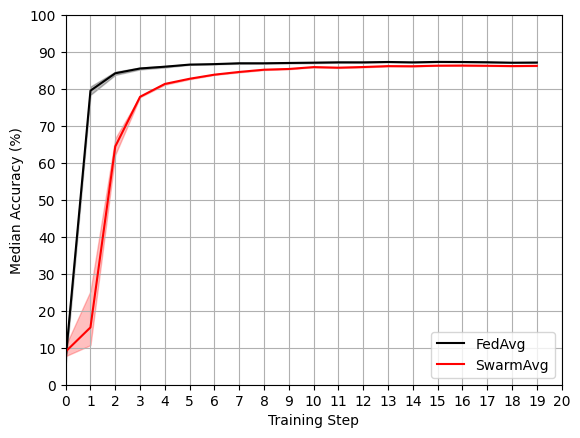
\includegraphics[width=\textwidth]{aeg_dense_1000}
		\caption{Full Graph}
	\end{subfigure}
	\begin{subfigure}{0.49\textwidth}
		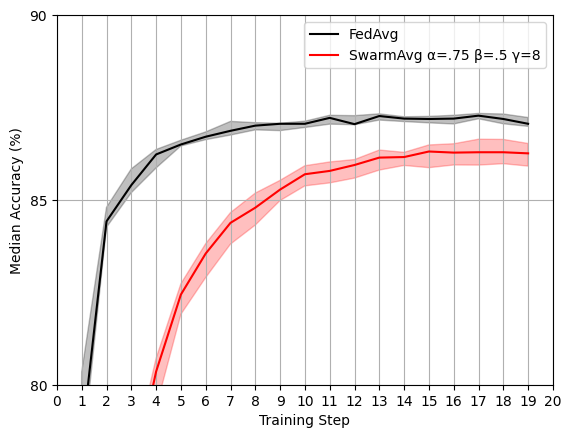
\includegraphics[width=\textwidth]{aeg_dense_1000_z}
		\caption{Zoomed Graph}
	\end{subfigure}
	\caption{Median accuracy by training step across 5 repeats. Each node has 1000 random data samples from MNIST-F. The shaded region represents the upper and lower quartile.}
	\label{aeg1}
\end{figure}

The results depicted in Figure \ref{aeg2} demonstrate that the SwarmAvg algorithm exhibits a slower convergence rate compared to FedAvg, trailing by at least 1 epoch for the duration of the test. Despite this, both methods ultimately achieve a similar level of accuracy, with less than a percent difference.

\begin{figure}[H] 
	\center{\textbf{Accuracy by Training Step for 100 Samples}} \\
	\begin{subfigure}{0.49\textwidth}
		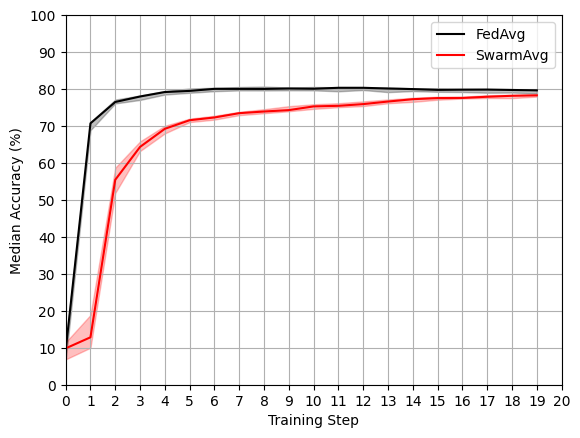
\includegraphics[width=\textwidth]{aeg_dense_100}
		\caption{Full Graph}
	\end{subfigure}
	\begin{subfigure}{0.49\textwidth}
		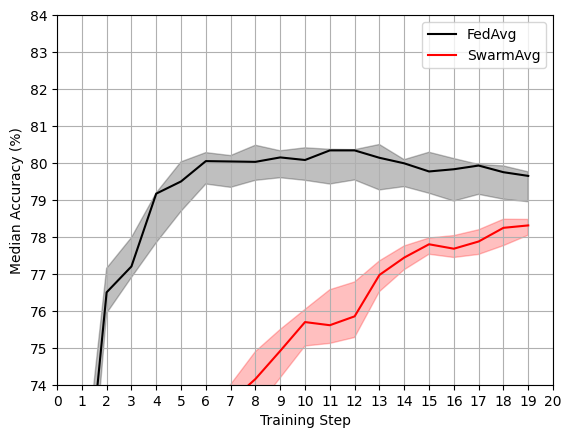
\includegraphics[width=\textwidth]{aeg_dense_100_z}
		\caption{Zoomed Graph}
	\end{subfigure}
	\caption{Median accuracy by training step across 5 repeats. Each node has 100 random data samples from MNIST-F. The shaded region represents the upper and lower quartile.}
	\label{aeg2}
\end{figure}


\begin{figure}[H] 
	\center{\textbf{Accuracy by Training Step for 25 Samples}} \\
	\begin{subfigure}{0.49\textwidth}
		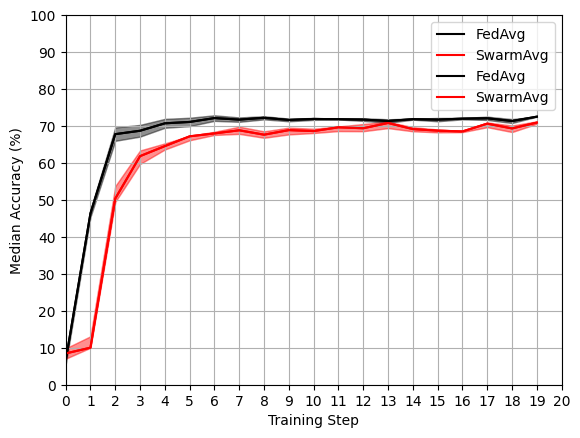
\includegraphics[width=\textwidth]{aeg_dense_25}
		\caption{Full Graph}
	\end{subfigure}
	\begin{subfigure}{0.49\textwidth}
		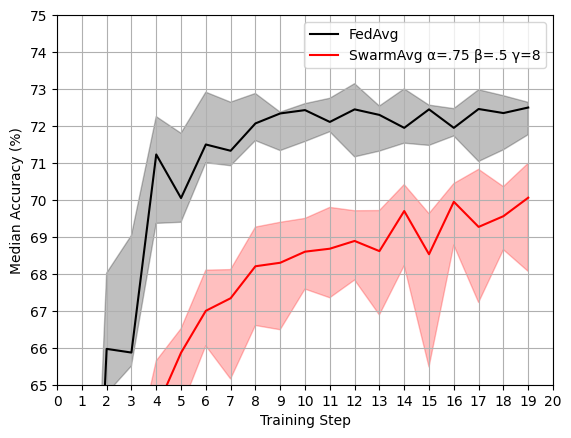
\includegraphics[width=\textwidth]{aeg_dense_25_z}
		\caption{Zoomed Graph}
	\end{subfigure}
	\caption{Median accuracy by training step across 5 repeats. Each node has 25 random data samples from MNIST-F. The shaded region represents the upper and lower quartile.}
	\label{aeg3}
\end{figure}

The trend of SwarmAvg ending with a lower accuracy than FedAvg continues in Figure \ref{aeg3}. Both algorithms also have a much lower accuracy than what they achieved previously, due to the drastic decrease in available data.

Similarly to Figure \ref{aeg2}, Figure \ref{aeg3} shows that SwarmAvg concludes with a lower accuracy than FedAvg. Furthermore, both algorithms exhibit a considerable decline in accuracy when compared to their previous performances with higher volumes of data. \\


The most noticeable impact resulting from reducing the volume of data is the significant decrease in the accuracy of both algorithms, as expected. However, it is also evident that the reduction in data affects SwarmAvg and FedAvg to a similar degree, as both of their peak accuracies stay within a similar range of each other in all tests. The difference in peak accuracy between the two algorithms was quite small, often within a 2 percent margin. \\

One of the prominent challenges associated with SwarmAvg is its slower convergence rate compared to FedAvg, particularly from the outset. SwarmAvg consistently takes a longer time to attain its peak accuracy. This may be attributed to the asynchronous nature of the nodes in SwarmAvg, which implies that some nodes that conduct training before others may have lower accuracy than expected. \\

It is worth noting that in all these evaluations, SwarmAvg has a slightly higher inter-quartile range than FedAvg, indicating that FedAvg is more consistent in terms of accuracy. However, this difference is minor. \\

One interesting feature of both SwarmAvg and FedAvg is that both algorithms seem to be affected by overfitting much less what would be expected. Especially with just 25 data samples per node, the effects of overfitting would usually be far more severe in a single node. However, this does not mean that the algorithms do not overfit, but it may indicate that the process of overfitting for both algorithms is drastically slowed down.

\section{Scenario 2: Sparsely Connected Network}
In reality, it is uncommon for each node to be linked with every other node. To simulate a more realistic scenario, a technique was employed to generate a network of nodes with a specific number of connections. When density is set to 0, the network is minimally linked, meaning that each node has at least one indirect path to every other node, but the minimal number of connections required to accomplish this exist. When density is set to 1, all nodes are connected to one another in a dense fashion. Since this measure may not provide a straightforward indicator of network density, two additional metrics will be provided:  Mean Minimum Hops (MMH) and Mean Connections per Node (MCPN). MMH denotes the mean minimum number of transitions required to get from one node to another in the network. MCPN denotes the average number of connections a given node possess, for a network of 10 nodes. \\

In order to conduct thorough testing on a variety of potential deployment scenarios, several different densities were tested for each count of data. The densities that were tested, along with their corresponding MMH and MCPN, are presented in Table \ref{sparsedensities}.

\begin{table}[H]
	\centering
	\begin{tabular}{l|l|l}
		Density & MMH & MCPN \\ \hline
		1 & 1.0 & 9.0 \\
		0.75    & 1.2 & 7.2  \\
		0.5    & 1.4 & 5.4  \\
		0.25    & 1.7 & 3.6  \\
		0    & 3.0 & 1.8  \\
	\end{tabular}
	\caption{The statistics for different density levels} \label{sparsedensities}
\end{table}

In order to assist the reader with visualizing the various density levels, some sample networks that were generated for each density can be found in Figure \ref{densefig}.

\begin{figure}[H]
	\centering
	\begin{subfigure}[b]{0.3\textwidth}
		\centering
		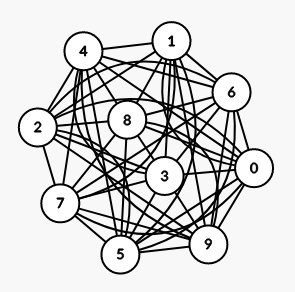
\includegraphics[width=\textwidth]{sparsegraph100}
		\caption{$density=1.0$}
	\end{subfigure}
	\begin{subfigure}[b]{0.3\textwidth}
		\centering
		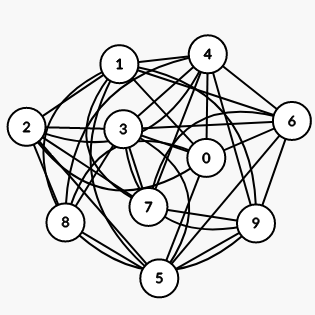
\includegraphics[width=\textwidth]{sparsegraph75}
		\caption{$density=0.75$}
	\end{subfigure}
	\begin{subfigure}[b]{0.3\textwidth}
		\centering
		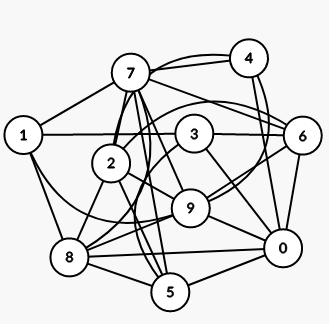
\includegraphics[width=\textwidth]{sparsegraph50}
		\caption{$density=0.5$}
	\end{subfigure}
	\begin{subfigure}[b]{0.3\textwidth}
		\centering
		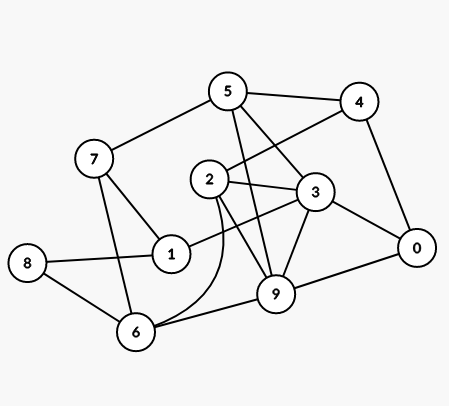
\includegraphics[width=\textwidth]{sparsegraph25}
		\caption{$density=0.25$}
	\end{subfigure}
	\begin{subfigure}[b]{0.3\textwidth}
		\centering
		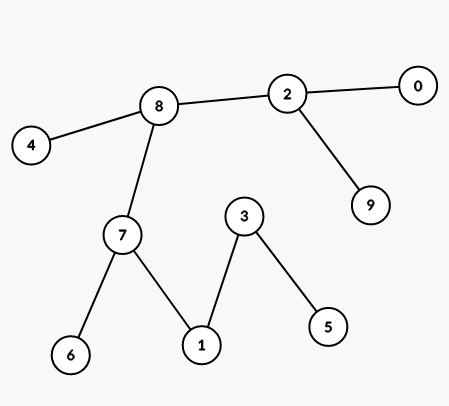
\includegraphics[width=\textwidth]{sparsegraph0}
		\caption{$density=0.0$}
	\end{subfigure}
	\caption{Example networks of nodes generated for each density level, visualised using the tool at \emph{https://csacademy.com/app/graph\_editor}. Each time a simulation is started, a new random network is generated for that simulation. \label{densefig}}
{}\end{figure}


This section does not include any testing of FedAvg. In scenarios where not every node is directly connected to the server node, FedAvg has two potential options: ignore all nodes which are not directly connected, or attempt to relay the model updates through connected nodes. As mentioned in Section \ref{relay}, relaying may not always be the optimal solution. Ignoring nodes is also not a good option, as data is wasted. Therefore, in this test, the decision was made to solely evaluate SwarmAvg.


\subsection{Sparse Network Results}
Below are results obtained from testing. The density of each line on the graph is indicated by the colour, with a green hue representing higher density and a red hue indicating lower density. For all tested densities, the value of $\gamma$ was set to $round_{down}(MCPN) - 1$, which ensures that each node can progress only after waiting for all but one of its neighbours. Notably, failure to reduce $\gamma$ for less dense networks would cause several nodes to wait for a number of neighbours that cannot be achieved. Due to the random nature of the graph generation, there will still be some nodes who have less than $\gamma$ neighbours, but this should be rare and the loop to wait for $\gamma$ neighbours will terminate after a certain number of tries anyway, ensuring that training can progress.

\begin{figure}[H] 
	\center{\textbf{Accuracy by Training Step for 1000 Samples, with Varying Density}} \\
	\begin{subfigure}{0.49\textwidth}
		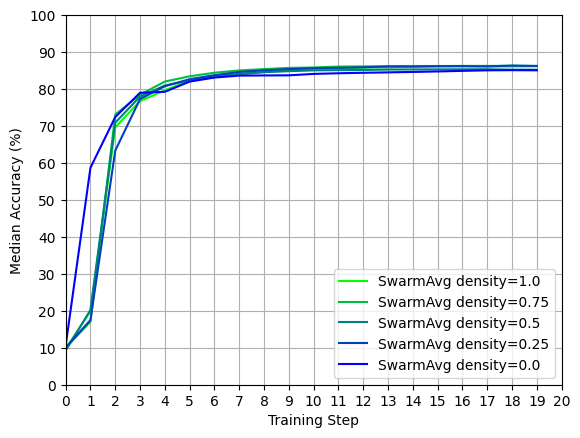
\includegraphics[width=\textwidth]{aeg_sparse_1000}
		\caption{Full Graph}
	\end{subfigure}
	\begin{subfigure}{0.49\textwidth}
		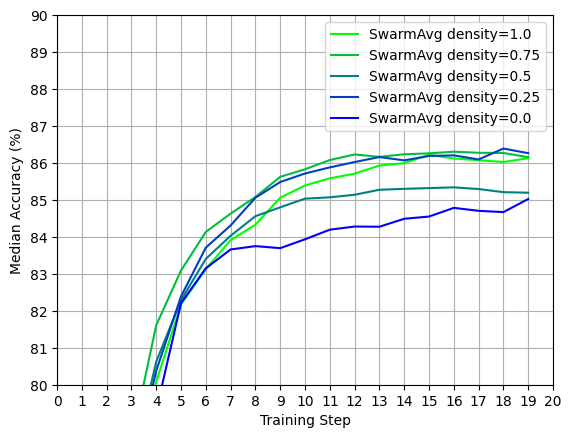
\includegraphics[width=\textwidth]{aeg_sparse_1000_z}
		\caption{Zoomed Graph}
	\end{subfigure}
	\caption{Median accuracy by training step across 5 repeats. Each node has 1000 random data samples from MNIST-F. Quartiles are not shown.}
	\label{aeg4}
\end{figure}

An observation that can be made of Figure \ref{aeg4} is that the different network densities perform very similarly. The final accuracy for all of the tests fell within a 2 percent range,  with the higher densities occupying the higher end. \\

One interesting feature of the Figure \ref{aeg4} is that the lowest density demonstrates faster convergence initially that the other densities. The author hypothesises that this may be due to groups of nodes forming local sub-networks which converge on their own sub-sets of data faster, but more slowly combine into the network as a whole as training progresses.

\begin{figure}[H] 
	\center{\textbf{Accuracy by Training Step for 100 Samples, with Varying Density}} \\
	\begin{subfigure}{0.49\textwidth}
		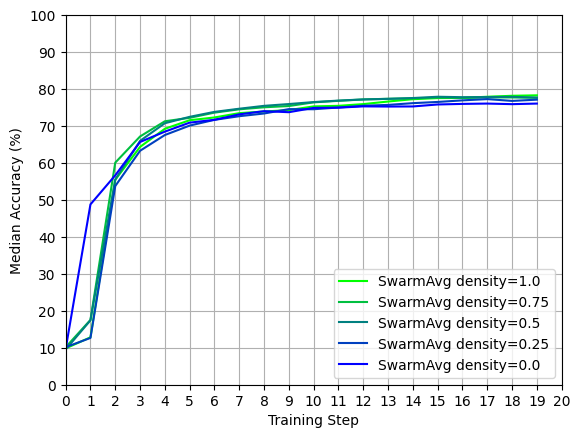
\includegraphics[width=\textwidth]{aeg_sparse_100}
		\caption{Full Graph}
	\end{subfigure}
	\begin{subfigure}{0.49\textwidth}
		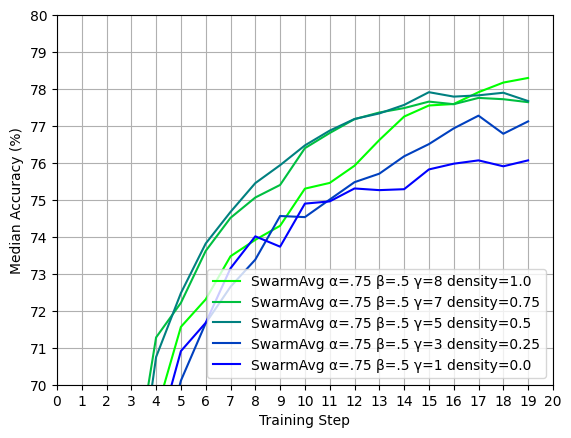
\includegraphics[width=\textwidth]{aeg_sparse_100_z}
		\caption{Zoomed Graph}
	\end{subfigure}
	\caption{Median accuracy by training step across 5 repeats. Each node has 100 random data samples from MNIST-F. Quartiles are not shown.}
	\label{aeg5}
\end{figure}

In Figure \ref{aeg5}, there is a greater spread of final accuracies, about 2.5 percent, than is shown in Figure \ref{aeg4}. The more noticeable feature of Figure \ref{aeg5} is that the final accuracies of all densities are approximately 8 percent lower than their counterparts with more data available in figure \ref{aeg4}.

\begin{figure}[H] 
	\center{\textbf{Accuracy by Training Step for 25 Samples, with Varying Density}} \\
	\begin{subfigure}{0.49\textwidth}
		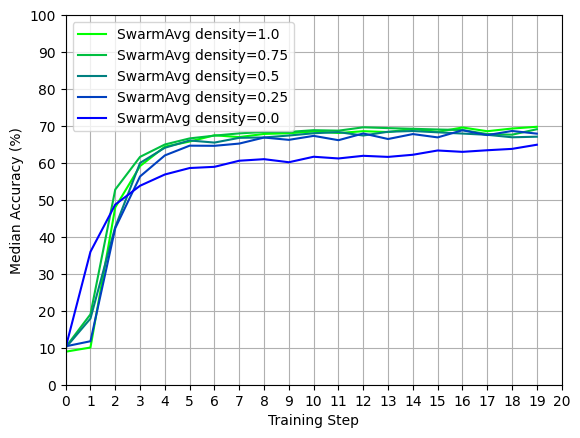
\includegraphics[width=\textwidth]{aeg_sparse_25}
		\caption{Full Graph}
	\end{subfigure}
	\begin{subfigure}{0.49\textwidth}
		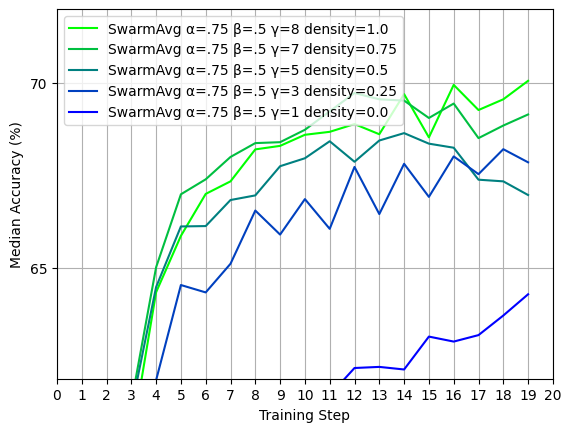
\includegraphics[width=\textwidth]{aeg_sparse_25_z}
		\caption{Zoomed Graph}
	\end{subfigure}
	\caption{Median accuracy by training step across 5 repeats. Each node has 25 random data samples from MNIST-F. Quartiles are not shown.}
	\label{aeg6}
\end{figure}

With 25 data samples, the tests depicted in Figure \ref{aeg6} show a much higher variation in final accuracies than the previous two figures. There is also a much higher degree of noise in this figure than any other, suggesting that training may be much less stable with this small number of data samples to train on.

It should also be noted that the lowest density is still exhibiting the behaviour of outperforming the other densities in the initial steps, however it appears that this effect has become slightly less prominent. \\


Generally, altering the network density of nodes has a small impact on the training of the nodes within the network. Decreasing the density of nodes typically leads to a lower final accuracy. This effect becomes more noticeable as the data volume provided to each node decreases, as demonstrated by the increased variability in training displayed in Figure \ref{aeg6} in comparison to Figures \ref{aeg4} and \ref{aeg5}. \\

The networks possessing a density of 0 attain their optima at a faster rate than those with higher densities. Figure \ref{aeg6} illustrates that the lower densities reach convergence marginally quicker than higher densities, yet are surpassed by the latter towards the end of training.

\section{Scenario 3: Densely Connected Network with Class Restrictions}

Decentralized machine learning algorithms, such as FedAvg and SwarmAvg, commonly involve a scenario where each node possesses a dataset whose distribution does not align with the overall data distribution across all nodes. In order to simulate such a scenario, a situation was created where each node was given access a unique set of three out of ten classes of MNIST-F. The tests in this experiment were conducted in a densely connected network of nodes, thereby allowing the evaluation of FedAvg as well.

\subsection{Dense Network with Class Restrictions Results}

\begin{figure}[H] 
	\center{\textbf{Accuracy by Training Step for 1000 Samples of 3 Classes}} \\
	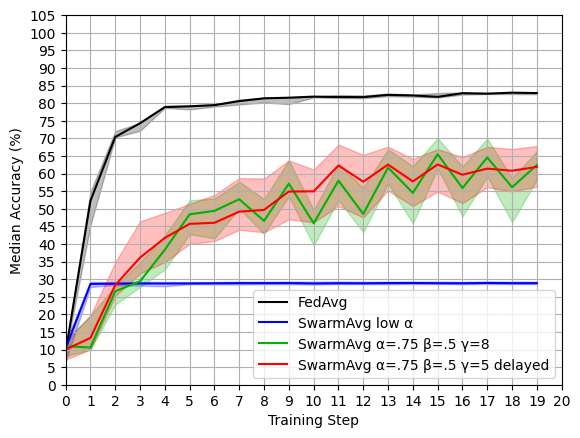
\includegraphics[width=0.49\textwidth]{aeg_unev_1000}
	\caption{Median accuracy by training step across 5 repeats. Each node has 1000 random data samples from MNIST-F. Quartiles are depicted as the shaded area. Each node has access to a unique set of 3 classes out of 10}
	\label{aeg7}
\end{figure}

During the course of the experiment, it was determined that SwarmAvg required some adjustments in order to function properly. One issue was a significant fluctuation in accuracy during the training process, which may have been due in part to the synchronization of nodes in the network. To address this concern, the decision was made to decrease the value of $\gamma$ and introduce a delay in the node start times, in order to desynchronize their training. The chosen delay time was 2 seconds. Figure \ref{aeg7} illustrates these two techniques, with the delayed training and reduced gamma method depicted in red, and the original method depicted in green. Evidently, these adjustments had a positive impact in minimizing the oscillations, although they were not entirely eliminated. \\

While attempting to adjust the parameters, another issue was encountered was divergent training, which occurs when nodes begin to learn completely separate models and start to disregard the models of their neighbours. It was observed that a low value of $\alpha$ was sufficient to cause this problem. When divergent training occurred, the nodes failed to achieve an accuracy level higher than 30 percent, which is expected if a node only trains on three out of the ten available classes. This effect is shown as the blue line of Figure \ref{aeg7}. \\

It is evident that SwarmAvg consistently exhibits a significantly lower level of accuracy compared to FedAvg. Additionally, the inter-quartile range of SwarmAvg is noticeably higher.

\begin{figure}[H] 
	\center{\textbf{Accuracy by Training Step for 100 and 25 Samples, with 3 Classes}} \\
	\begin{subfigure}{0.49\textwidth}
		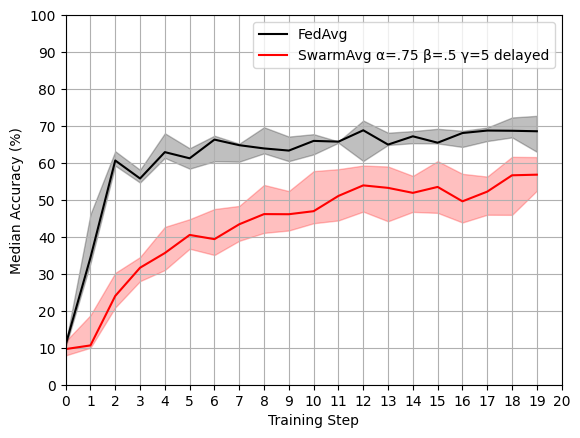
\includegraphics[width=\textwidth]{aeg_unev_100}
		\caption{Samples=100}
	\end{subfigure}
	\begin{subfigure}{0.49\textwidth}
		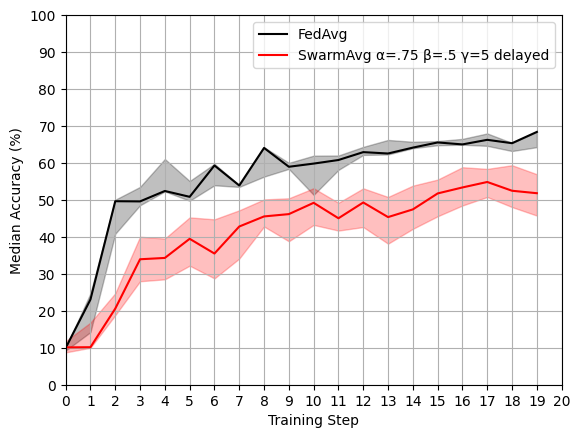
\includegraphics[width=\textwidth]{aeg_unev_25}
		\caption{Samples=25}
	\end{subfigure}
	\caption{Median accuracy by training step across 5 repeats. Quartiles are depicted as the shaded area. Each node has access to a unique set of 3 classes out of 10}
	\label{aeg8}
\end{figure}

When performing training on a lower sample count, as depicted in Figure \ref{aeg8}, the oscillations in SwarmAvg seem to have been drastically reduced when compared to \ref{aeg7}. However, both SwarmAvg and FedAvg have lower accuracies by the end of training than they did with 1000 samples. \\

It is clear that the reduction of data volume per node has a detrimental impact on the performance of SwarmAvg in general. However, in these restricted class tests, this effect is less pronounced compared to previous tests where each node had access to all possible classes. It should be noted that SwarmAvg encounters accuracy oscillations, which can be partially attributed to the synchronized training steps of nodes. Nevertheless, by decreasing the value of $\gamma$ and staggering the startup of nodes, these oscillations can be mitigated. Moreover, reducing the data volume also seems to aid in reducing the effect of these oscillations, possibly implying that nodes are being trained excessively in a single step.

\section{Scenario 4: Sparsely Connected Network with Class Restrictions}
This scenario was designed to test the SwarmAvg algorithm to its limits. It not only involved limiting data to each node, but also limiting the classes each node had access to in the same fashion as Scenario 3, and also constraining the networks to be sparsely connected.

\subsection{Sparse Network with Class Restrictions Results}
\begin{figure}[H] 
	\center{\textbf{Accuracy by Training Step for 1000, 100 and 25 Samples, with 3 Classes and Varying Density}} \\
	\begin{subfigure}{0.49\textwidth}
		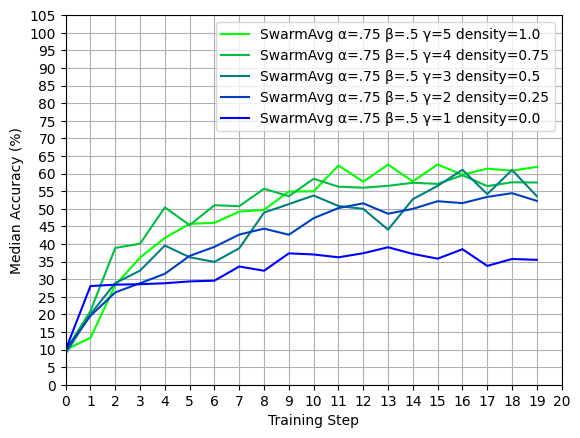
\includegraphics[width=\textwidth]{aeg_sparse_unev_1000}
		\caption{Samples=1000}
	\end{subfigure}
	\begin{subfigure}{0.49\textwidth}
		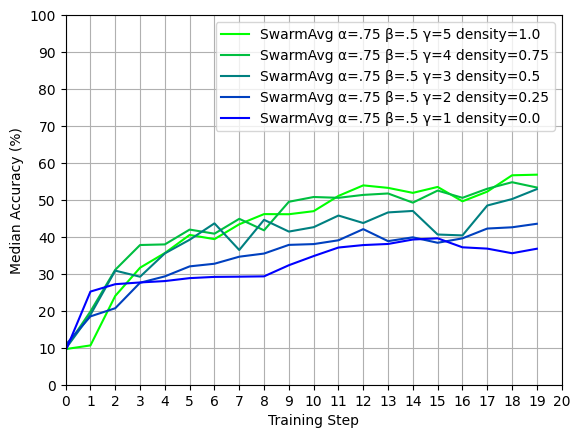
\includegraphics[width=\textwidth]{aeg_sparse_unev_100}
		\caption{Samples=100}
	\end{subfigure}
\begin{subfigure}{0.49\textwidth}
	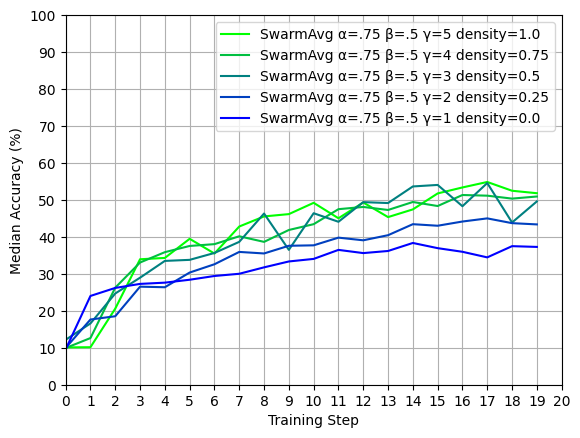
\includegraphics[width=\textwidth]{aeg_sparse_unev_25}
	\caption{Samples=25}
\end{subfigure}
	\caption{Median accuracy by training step across 5 repeats. Quartiles are not shown. Each node has access to a unique set of 3 classes out of 10.}
	\label{aeg9}
\end{figure}


In all three tests, it is clear that a higher density is highly correlated with higher performance in this scenario. It is also noteworthy that with a network density of 0, no matter which volume of data was presented, the accuracy curve was very similar. However, as the density of the network increased, so did the degree at which it was effected by the reduction in data. This scenario also presented graphs with a high degree of noise when compared to other scenarios, despite representing the median of 5 training runs. However, the level of noise is somewhat consistent on all three tests with different data volumes.
